\chapter{Literature Survey}

\section{The PUF concept}
The simplest sentence to describe PUF is "A PUF is an object's fingerprint" \cite{Reference4}. The fingerprint can represent a specific human in the world, such as the PUF can represent
an object. The fingerprint is inherently created when people was born, and the so does PUF, which is inherently exist in an object according to unique manufacturing random variation \cite{Reference4}.
With the representation and inherent property, the fingerprint and the PUF is said to be unclonable since it is impossible to control and predict human's fingerprint. This is an important concept for PUF. \par

This intrinsic property can be extract from chip which has PUF circuit existed inside \cite{Reference2}. The way PUF works is by entering a certain length of bits(so called challenge) into the PUF, and it will
generate another specific length of bits(so called response). According to the property of PUF that was discuss above, it is impossible to find two different PUF that will produce the same response when entering same challenge(See Figure \ref{fig:figure1}).
\begin{figure}[htp]
\centering
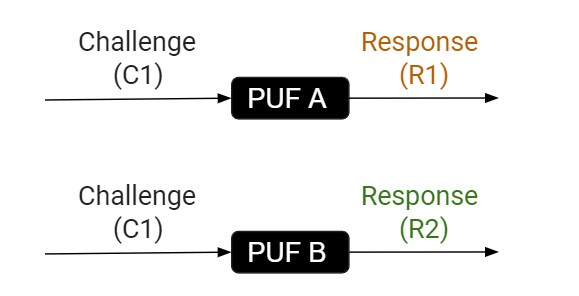
\includegraphics[width=8cm]{figures/figure1.jpg}
\caption{Different PUF that generate different response when input same challenge}
\label{fig:figure1}
\end{figure}

\section{Weak and strong PUF}
PUF can be classified into two categories, weak and strong PUF according to the strength of PUF. The strength of PUF indicate the number of challenge response pairs(so called CRPs) can be generate 
from the PUF \cite{Reference1}. The higher numbers of the CRPs can a PUF generate, the better strength it has. Generally, if increasing the size of the PUF leads to a linear increase in the number of CRPs, it is consider weak PUF. 
On the other hand, if increasing the size of the PUF leads to a exponential increase in the number of CRPs, it is consider strong PUF.\par

For the weak PUF, it represent the PUF that has smaller set of CRPs. While it is impossible to 
create a clone of PUF, but with small set of CRPs, this will allow attacker to record all the CRPs when attacker has physical access to PUF \cite{Reference1}. With the knowledge of CRPs, attacker can easily provide the corresponding
response to challenge as like they have a clone(See Figure \ref{fig:figure2}). The weak PUF can be use for authentication and key storage. However, since weak PUF's CRPs can be fully access, ensure having a secure environment and whether the original PUF is being evaluating is relatively important \cite{Reference1}.
\begin{figure}[htp]
    \centering
    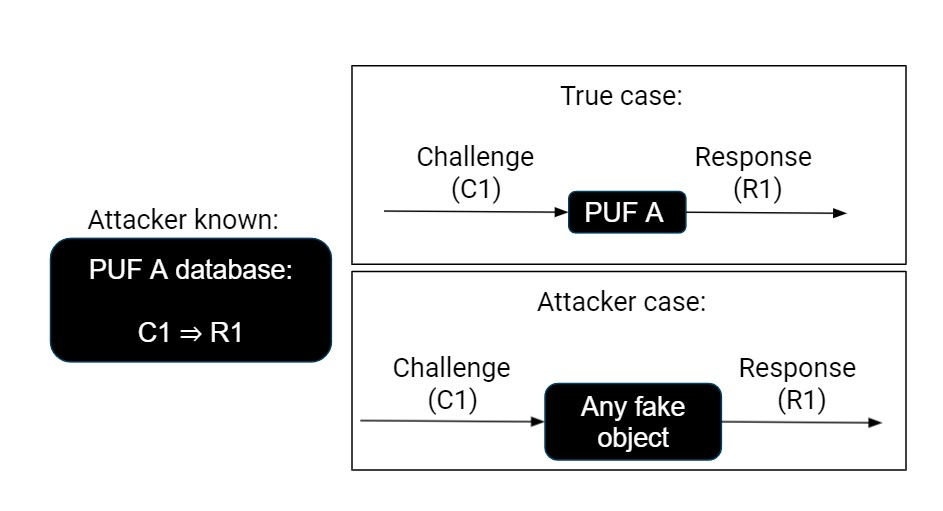
\includegraphics[width=10cm]{figures/figure2.jpg}
    \caption{Attacker can perform same behavior as Weak PUF when have fully access to CRPs and not under secure environment}
    \label{fig:figure2}
    \end{figure}

For strong PUF, means the number of CRPs is significantly large that even attacker get access, having throughout knowledge of CRPs is impossible. While the number of CRPs is so large,
and the CRP are randomly selected in usage, the probability that attacker has knowledge about the CRP currently using is small. In addition, each CRPs that is used once will 
be discarded(See Figure \ref{fig:figure3}) so even if attacker recorded certain CRPs, also called eavesdropped, they will not be able to put them into use. The strong PUF can also be use for authentication but do not need to protect CRPs
as serious as weak PUF.

\begin{figure}[htp]
    \centering
    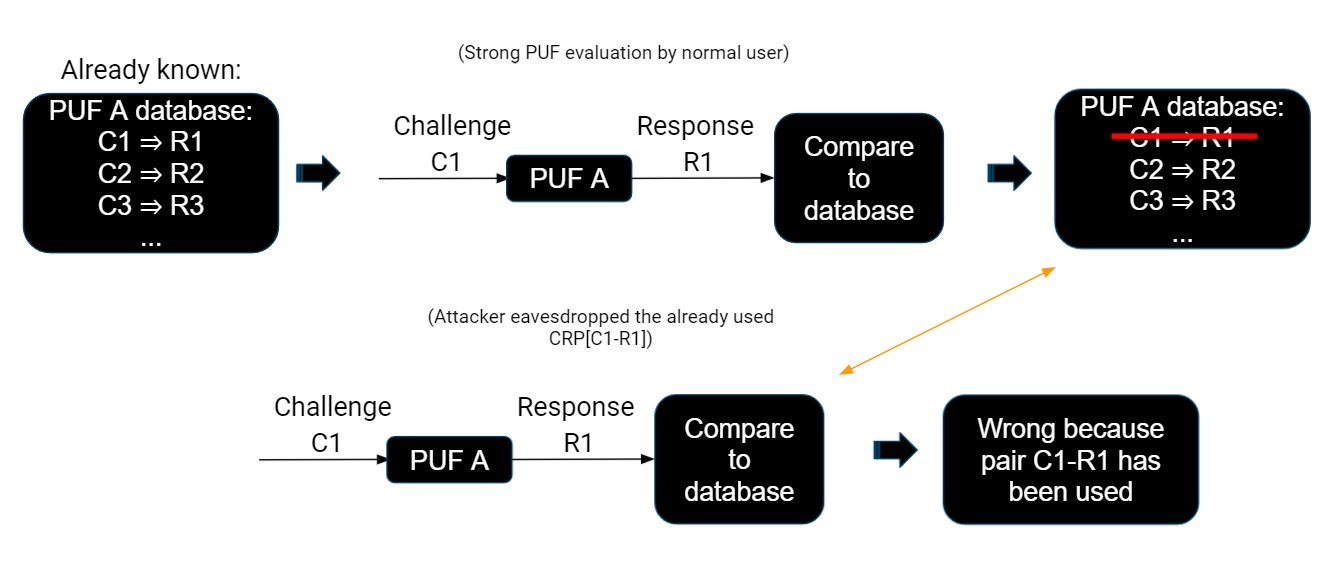
\includegraphics[width=15cm]{figures/figure3.jpg}
    \caption{The attacker eavesdropped CRP that has been used can not successfully validate in next evaluation for strong PUF}
    \label{fig:figure3}
    \end{figure}

\section{Authentication}
One of the application of PUF is authentication. As discuss in Chapter 1's introduction, PUF does not require huge computational power and are cost effective, so it is suitable for many devices,
especially the resources-constraint devices. The PUF's authentication included two stages, enrollment and authentication stage. In the enrollment stage, the company possess the PUF, so
company can connect server to PUF and sent lots of challenges along with recording the CRPs into the database \cite{Reference2} (See Figure \ref{fig:figure4}).

\begin{figure}[htp]
    \centering
    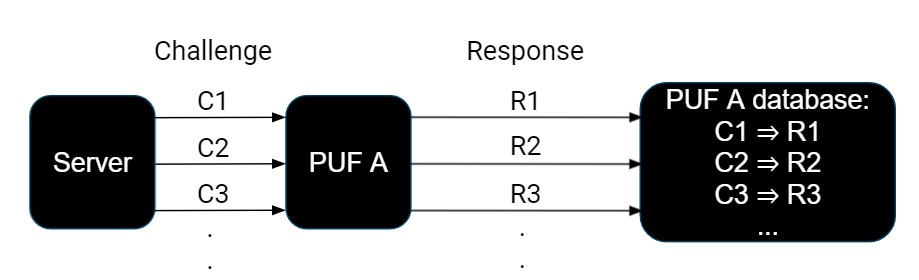
\includegraphics[width=8cm]{figures/figure4.jpg}
    \caption{Enrollment stage in PUF authentication}
    \label{fig:figure4}
    \end{figure}

After recording all the CRPs, the company can now implement PUF on electronic devices.
In the authentication stage, the server sent arbitrary challenge to the devices that contain PUF while the device will return response. Afterward, the server compare the response from the device with the database, 
if the challenge and response pair exist in the database, the device is valid \cite{Reference2} (See Figure \ref{fig:figure5}). A life example will be banking card.

\begin{figure}[htp]
    \centering
    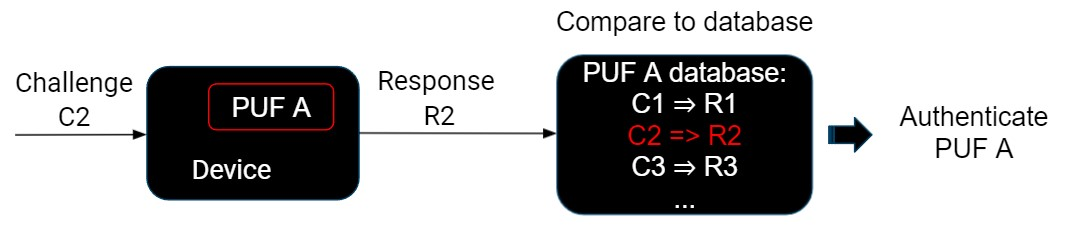
\includegraphics[width=8cm]{figures/figure5.jpg}
    \caption{Authentication stage in PUF authentication}
    \label{fig:figure5}
    \end{figure}

\section{Arbiter PUF and XOR arbiter PUF}
There are many different types of PUF such as arbiter PUF, ring oscillator PUF, lightweight PUF, etc. In this paper, arbiter PUF and its mutation will be introduced in detail. The general idea of
the arbiter PUF is comparing the transition speed for two electrical signal in the PUF's structure(See Figure \ref{fig:figure6}). The arbiter PUF's structure contains a numbers of 
multiplexers and a arbiter(mostly D flipflop), and two multiplexers will combined into a switching box \cite{Reference3}. Look at Figure \ref{fig:figure6}, when enter a challenge bits, apply each challenge bit to a switching box, bit 1 indicate the upper and lower signal will switch 
while bit 0 indicate the two signals remain unchanged in each switching box. This will eventually form paths for the signals. Then the signals start transferring, the time arrived at the arbiter for two signals 
is different since each multiplexer and wire has unique delay. The arbiter will determine which path is faster and based on that response a binary bit, if upper path is faster, the response is 1, 
otherwise the response is 0. \par

The arbiter at the end is always fair, which will not favor any one of the path. Even there exist bias, a simple solution of adding a delay in the structure can solve the problem. For example, if the arbiter favor the lower path,
by adding a delay to upper path, it can has a head start. By looking at the Figure \ref{fig:figure6}, it is clear that the CRPs will be exponential. Assuming there are n switching boxes, two possible cases in each switching box, so the 
number of CRPs is $2^{n}$, which indicate the arbiter PUF is a strong PUF. Arbiter PUF can also return longer response by input K different challenges and get a K bits response.

\begin{figure}[htp]
    \centering
    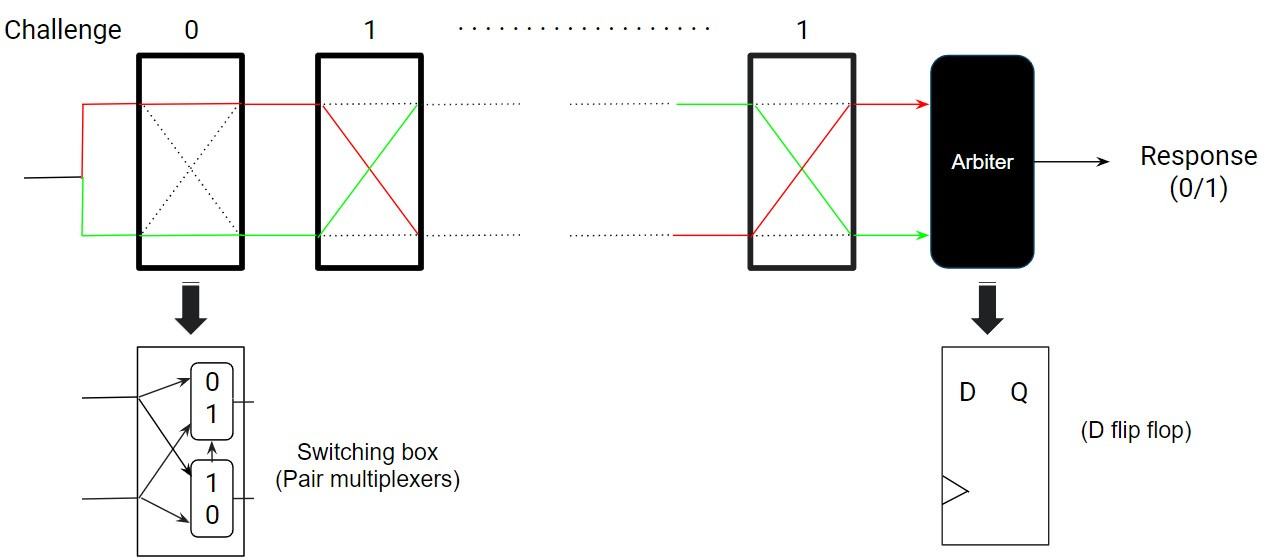
\includegraphics[width=12cm]{figures/figure6.jpg}
    \caption{Arbiter PUF structure}
    \label{fig:figure6}
    \end{figure}

The normal arbiter PUF is vulnerable to modeling attack, the propose of XOR arbiter PUF is to increase the robustness of arbiter PUF. The basic concept is to integrated multiple parallel arbiter PUF, given same challenge to each arbiter PUF and XORed each response to produce final response(See Figure \ref{fig:figure7}) \cite{Reference5}.
According to simulation, in book \cite{Reference4} provides the XOR arbiter PUF will have nonlinearity property that makes it harder to model.

\begin{figure}[htp]
    \centering
    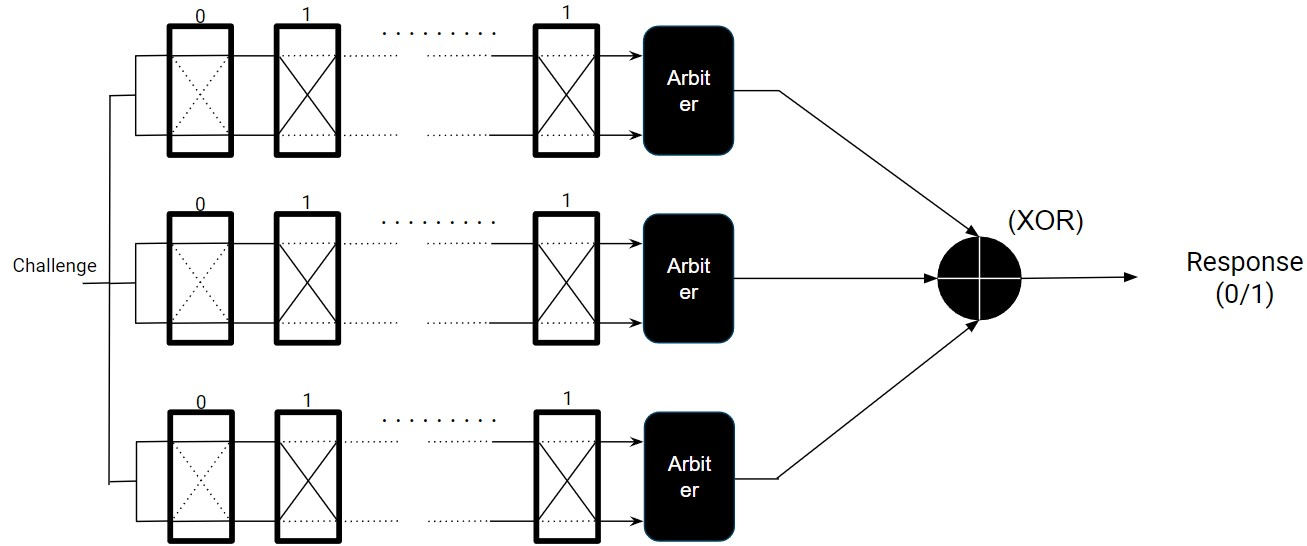
\includegraphics[width=12cm]{figures/figure7.jpg}
    \caption{XOR arbiter PUF structure}
    \label{fig:figure7}
    \end{figure}

\section{Modeling attack on PUF}
Many different threat can perform on devices, such as eavesdropped, gain access to the memory that store secret keys. For PUF, the main threat is that attacker can use technique 
like machine learning to simulate the behavior of CRPs(so called modeling), which means even without the devices, attacker can still response correctly when a challenge is 
provided. Take arbiter puf as example, assume an arbiter PUF with i switching box, and the challenge apply to each switching box is c[i]. The two signal travel through the 
the path determine by challenge, and arrive at the arbiter in different time because of the delay in each component. The final response depend on the sign of final delay 
difference:
\begin{equation}
    r =\begin{cases}
    1, & \text{if $\Delta c<0$}.\\
    0, & \text{otherwise}.
    \end{cases}
\end{equation}
which the delay difference is calculated by subtract the upper path with lower path's delay. The final delay difference $\Delta c$ can represent as $w^{T}\Phi$, where $w^{T}$ is 
a weight vector that represent delays for the components in PUF, and $\Phi$ is the applied i bits challenge \cite{Reference5}. $w^{T}\Phi = 0$ will provide a hyperplane that separate the space for $\Phi$, one side of the hyperplane are predict as having response 1, the other side of the hyperplane
are predict as having response -1. In conclusion, the correct hyperplane indicate the good prediction of PUF. Machine learning such as logistic regression can play the role well. The modeling result for a arbiter PUF with 64 switching boxes, 
by using the logistic regression can get a good performance of 99.9\% in very short time with 18050 training CRPs \cite{Reference6}.

For the XOR arbiter PUF, it is also possible to use logistic regression to predict the behavior but will be harder.

\section{Reconfigurability of PUF}
In order to alleviate the problem that PUF is vulnerable to modeling attack, reconfiguration property embedded on PUF has been proposed. For example, the one-time-PUF(so called 
OPUF), the general idea is that the its configuration alter after every authentication session, which means CRPs behavior of the PUF is changed and invalidate the modeling attack. This is based on the
forward unpredictability and backward unpredictability properties that OPUF possess \cite{Reference7}. In Figure \ref{fig:figure8} shows the concept of forward unpredictability and backward unpredictability.
The orange line represent the forward unpredictability, which will ensure the responses collected before the reconfiguration process is invalid afterward. As for the blue line, 
which represent backward unpredictability, it will ensure the pattern observed by attacker using modeling attack on PUF' is invalid for predicting the PUF before reconfiguration process. 
In this case, assume an attacker are performing a modeling attack on the PUF, and required certain amount of CRPs to gain proper prediction. However, the OPUF's structure keep changing every execution, which means the CRPs 
behavior is changing, so the modeling attack will can't be up to date or do mot have time to collect enough CRPs.
\begin{figure}[htp]
    \centering
    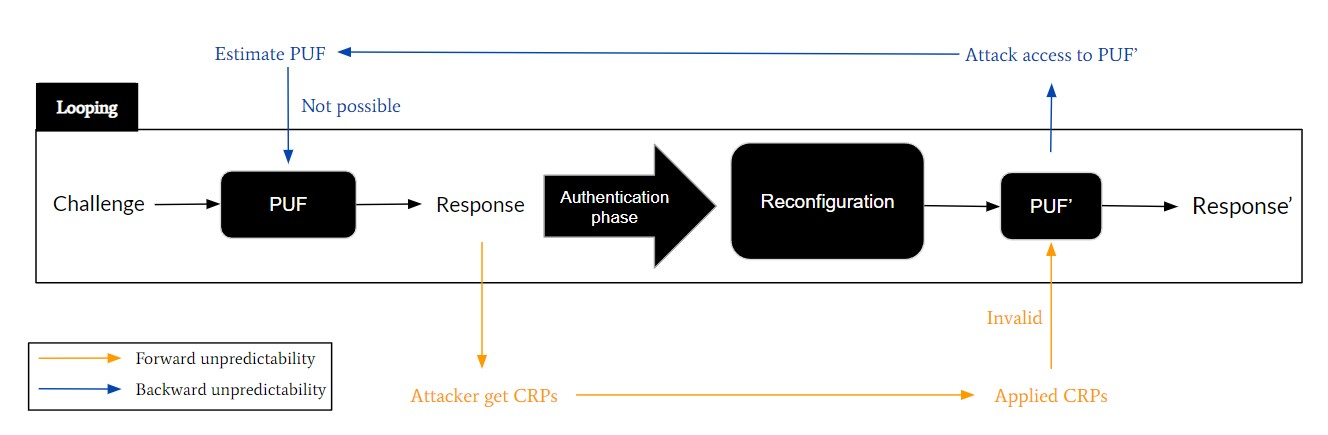
\includegraphics[width=14cm]{figures/figure8.jpg}
    \caption{Concept of forward unpredictability and backward unpredictability}
    \label{fig:figure8}
    \end{figure}

DPUF can be consider as an example for creating the OPUF, it is build up with bit cells which contain capacitors and transistors, each cell store information of value 0 and 1. However, these component will leak 
electrical signals every period of time, which means the behavior might be eavesdropped \cite{Reference7}. Therefore performing reconfiguration process every period of time is effective. The reconfigurability can be shown in Figure \ref{fig:figure9}, by varying parameters
such as refresh-pause interval and the memory block, where the former can cause random bit flip in the cells while the latter store final response in an random memory block 
which will alter every period of time, PUF can present unpredictable behavior that prevent from attacker perform modeling attack.

\begin{figure}[htp]
    \centering
    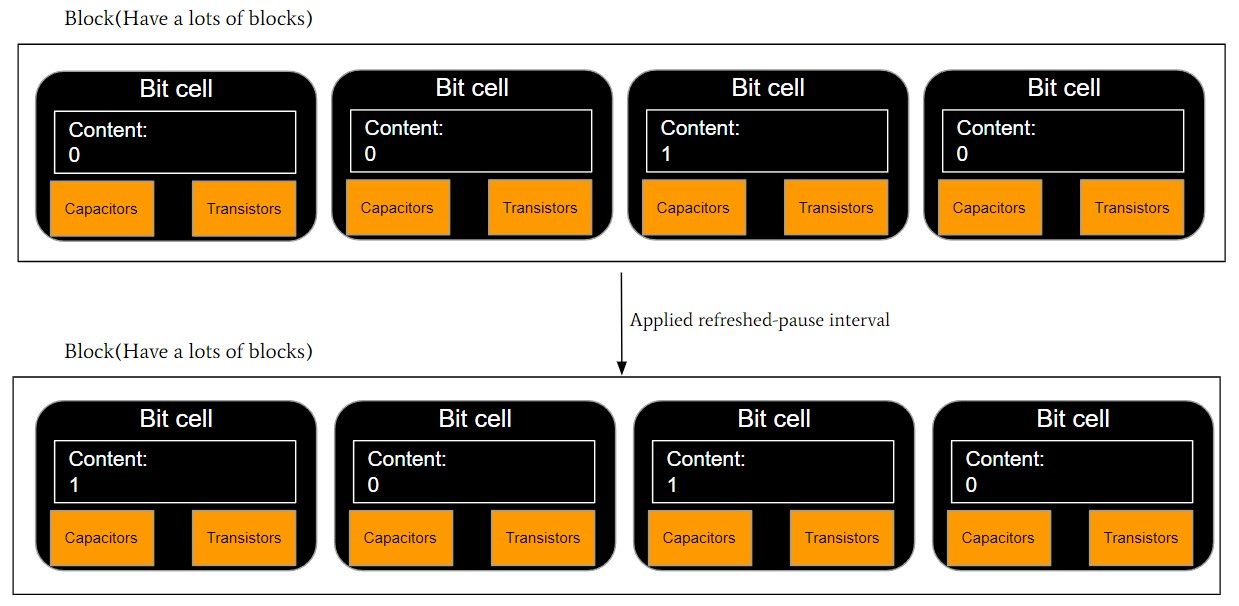
\includegraphics[width=10cm]{figures/figure9.jpg}
    \caption{Reconfigurability framework of DPUF}
    \label{fig:figure9}
    \end{figure}

\section{Summary}
In summary, chapter 2 describe PUF as a novel approach to increase the security robustness of electrical devices by making use of its unique physical characteristics and how it can be used
for devices authentication. Also, the working process and concepts for arbiter PUF and XOR arbiter PUF is introduced in detail. Last, largest potential threat on PUF called the modeling attack 
and its countermeasure are analyzed in details.